\chapter{ランサムウェア}
% 本章では,本研究の提案手法に関連する要素に注目して,ランサムウェアについて説明する.





\section{概要}
\label{sec:ransom-overview}
ランサムウェアとはマルウェアの一種であり,攻撃者が要求した金額が支払われるまで,システムやデータへのアクセスを制限する.
言い換えると,データや計算資源,サービスなどのリソースを人質に取って被害者を脅迫することで身代金を要求するマルウェアがランサムウェアである.

ランサムウェアはリソースへのアクセスを制限する方法に基づいて暗号化ランサムウェアとロッカーランサムウェアに分類される \cite{oz2022survey}.
暗号化ランサムウェアは感染先ホストのファイルやデータを暗号化し,元のファイルを削除または上書きする.
ロッカーランサムウェアは暗号化を行わず,デスクトップのスクリーンやブラウザをロックすることで被害者がシステムを利用できないようにする.
本研究は暗号化ランサムウェアを対象としているため,本稿では暗号化ランサムウェアを単に「ランサムウェア」と呼ぶことにする.

\begin{figure}[t]
  \begin{center}
    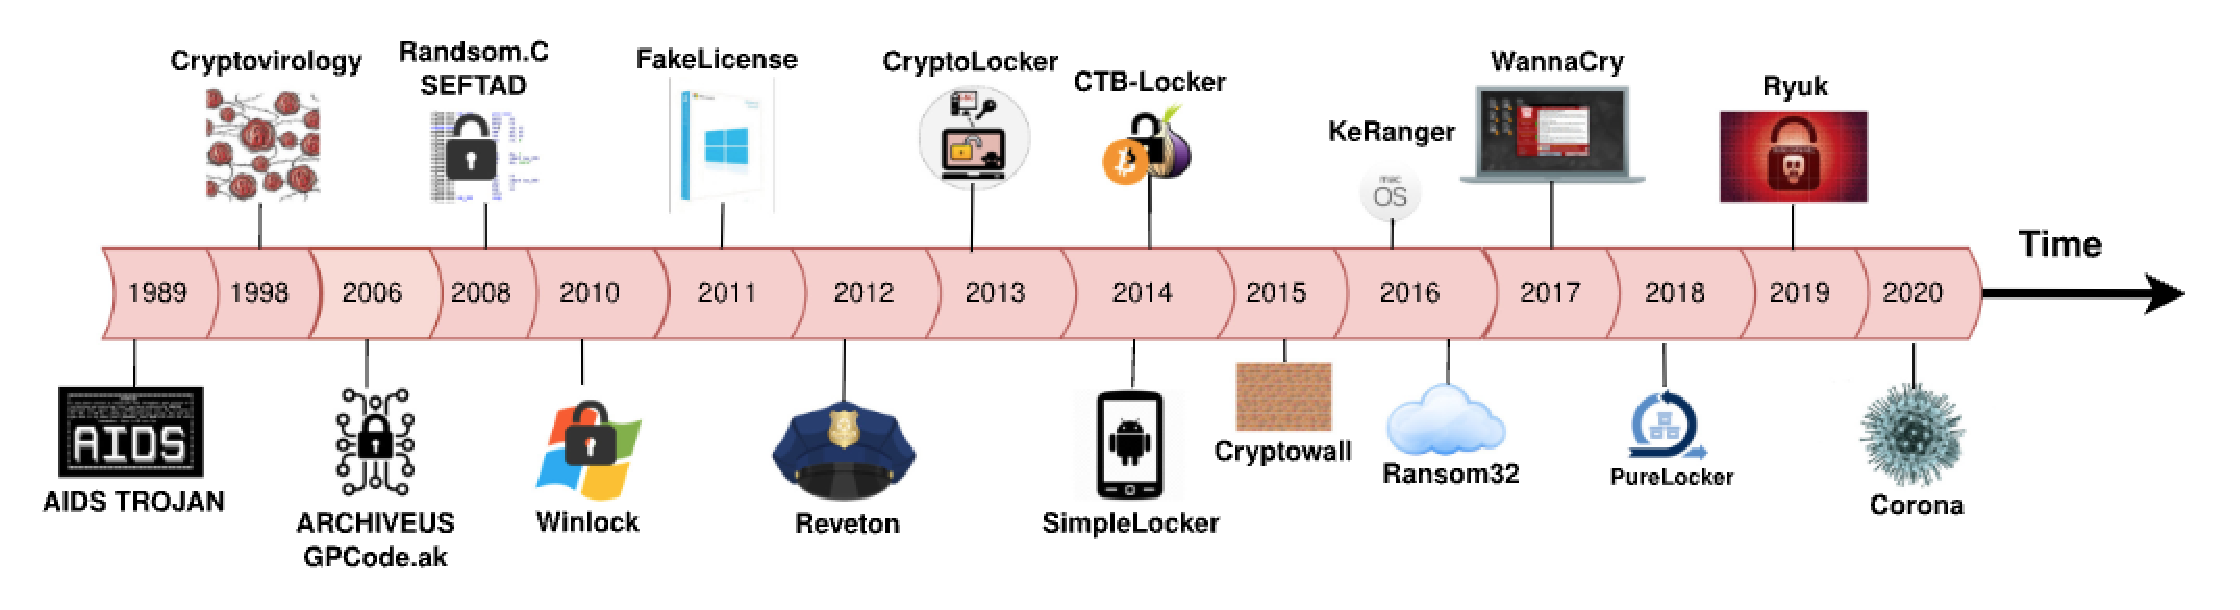
\includegraphics[width=\columnwidth]{doc/img/ransom-evolution.eps}
  \end{center}
  \caption{Development of major ransomware families (1989–2021). The first know ransomware, AIDS Trojan, was introduced in 1989. \cite{Evolution-Ransomware}.}
  \label{fig:ransom-evolution}
\end{figure}

\figref{fig:ransom-evolution}に示すように,AIDS Trojan \cite{aids-trojan} は1989年に最初のランサムウェアとして登場した.
AIDS Trojanは被害者に郵送されたフロッピーディスクを介して感染し,Windowsシステムを対象としていた.
その後インターネットの普及に伴い,ランサムウェアによる被害が増加し始めた.
2005年に登場したGPCode \cite{PGPCoder42:online} はフィッシングメールを介して感染し,独自の暗号化アルゴリズムによってファイルを暗号化した.

現代のランサムウェアはますます高度化している.
ランサムウェアの進化における重要な要素を以下に列挙する.
\begin{itemize}
  \item AESなどの対称鍵暗号化アルゴリズムやRSA,楕円曲線暗号などの非対称鍵暗号化アルゴリズムを使用して暗号化を行うようになっている \cite{Evolution-Ransomware}.
        これにより,復号鍵を入手することができなければデータの復号はほぼ不可能となった.

  \item Windowsだけでなく,Linux,macOS,Androidなどの他のOSを対象としたランサムウェアも登場するようになった.

  \item ビットコインに代表される仮想通貨が普及したことで身代金の支払いが匿名で行えるようになり,攻撃者の特定が難しくなった.

  \item ランサムウェアの開発と配布を有料で行うサービスであるRansomware as a Service (RaaS) が登場し,専門知識が無くとも容易に攻撃を実施することができるようになった.

  \item 無差別的な攻撃から,特定の高価値な組織 (政府機関や大企業など) を対象とした高度な攻撃に移行しつつある \cite{early-detection}.
\end{itemize}

\section{ランサムウェアの分類}
\subsection{悪意ある振る舞いに基づく分類}
\ref{sec:ransom-overview}節で述べたように,ランサムウェアは被害者が身代金を支払うまでリソースへのアクセスを制限するが,
アクセスを制限する方法には多様性が見られる.
本稿ではOzらの分類 \cite{Evolution-Ransomware} を参照し,その方法として\textbf{暗号化},\textbf{データ破壊},\textbf{データ窃取}を扱う.

暗号化:
ランサムウェアは暗号化鍵を用いてデータを暗号化し,元のデータを削除するか,暗号化後のデータで上書きする.
この時使用する鍵はランサムウェアの実行ファイルに埋め込まれているか,感染先ホスト上で生成されるか,C2サーバとの通信から取得されるかのいずれかである.
ファイルを暗号化するランサムウェアの中には,暗号化の対象とするファイルを限定するものも存在する.
例えばCTB-Locker \cite{ctb-locker} は,被害者にとってより高価値なファイルのみを暗号化するために,
.pdfや.zipなどの拡張子を持つファイルを暗号化対象としている.
また,Jigsaw \cite{byrne2017jigsaw} は10MB以下のファイルのみを暗号化する.
このように,ランサムウェアの一部は暗号化の対象とするファイルを限定することで,
ランサムウェアの活動が検出されるリスクを緩和している \cite{huang2017flashguard}と考えられる.

データ破壊:
破壊活動を目的としているがランサムウェアに擬態して攻撃者の意図を隠蔽しようとするマルウェアが確認されている.
例えば,2017年に発見されたNotPetya \cite{Petya-No22:online} は,ハードディスク全体を暗号化した後,
ビットコインの送金先として無効なアドレスを提示していた.
このアドレスはランダムに生成されており,攻撃者が金銭を回収する意図がないことから,
NotPetyaは破壊活動を目的として作成されたと考えられる \cite{Petya-No22:online}.
同様の攻撃として,暗号化を行わず,ランダムなデータでファイルを上書きするマルウェアを作成し使用することも可能である.
なお,このタイプのマルウェアの被害者は身代金を支払ってもリソースを復旧することができないが,
本研究ではランサムウェアとして扱う.

データ窃取:
ランサムウェアは機密文書や顧客の個人情報などの重要データを摂取する可能性がある.
データの暗号化または破壊とデータの窃取を組み合わせて脅迫を行うランサムウェアを「二重脅迫ランサムウェア」と呼ぶ.
二重脅迫ランサムウェアは,データの復旧のために一回,窃取したデータの公開を防ぐためにもう一回,被害者に身代金を要求する.
二重脅迫ランサムウェアによる被害は近年増加しており,SOPHOS社が発表したレポート \cite{sophos-report:online} によると,
2023年に発生したランサムウェアインシデントのうち32\%においてデータの摂取も発生している.
加えて,データの窃取のみによって脅迫を行う「ノーウェアランサム」\cite{nowhere-ransom} と呼ばれる手法も確認されている.

\subsection{暗号化アルゴリズムに基づく分類}
データを暗号化するランサムウェアは,ISO/IEC \cite{ISOIEC2784:online} などの標準化団体が採択した標準的なアルゴリズムを使用する場合と,
攻撃者によって独自に設計された暗号化アルゴリズムを使用する場合がある.
Begovicら \cite{begovic2023cryptographic} が調査した,1991年から2021年までに確認された著名なランサムウェア変種の
暗号化アルゴリズムの使用状況を\figref{fig:encrypt_algo}に示す.
\figref{fig:encrypt_algo}によると8.2\%のランサムウェアが独自の暗号化アルゴリズムを使用しているが,
近年のランサムウェアはAESやRSAといった標準的な暗号化アルゴリズムを使用する傾向が強いことがいくつかの先行研究 \cite{Evolution-Ransomware,key-management}にて指摘されており,
この数値には初期のランサムウェアが多く含まれていると考えられる.
より具体的には,攻撃者が独自に設計した暗号化アルゴリズムは強度が不十分で暗号解読者による解読が容易であることが多い \cite{key-management}ため,
2000年代後半から2010年代前半にかけて,十分に評価され強度が高い暗号化アルゴリズムが採用されるようになっていった \cite{Evolution-Ransomware}.

\begin{figure}[tb]
  \begin{center}
    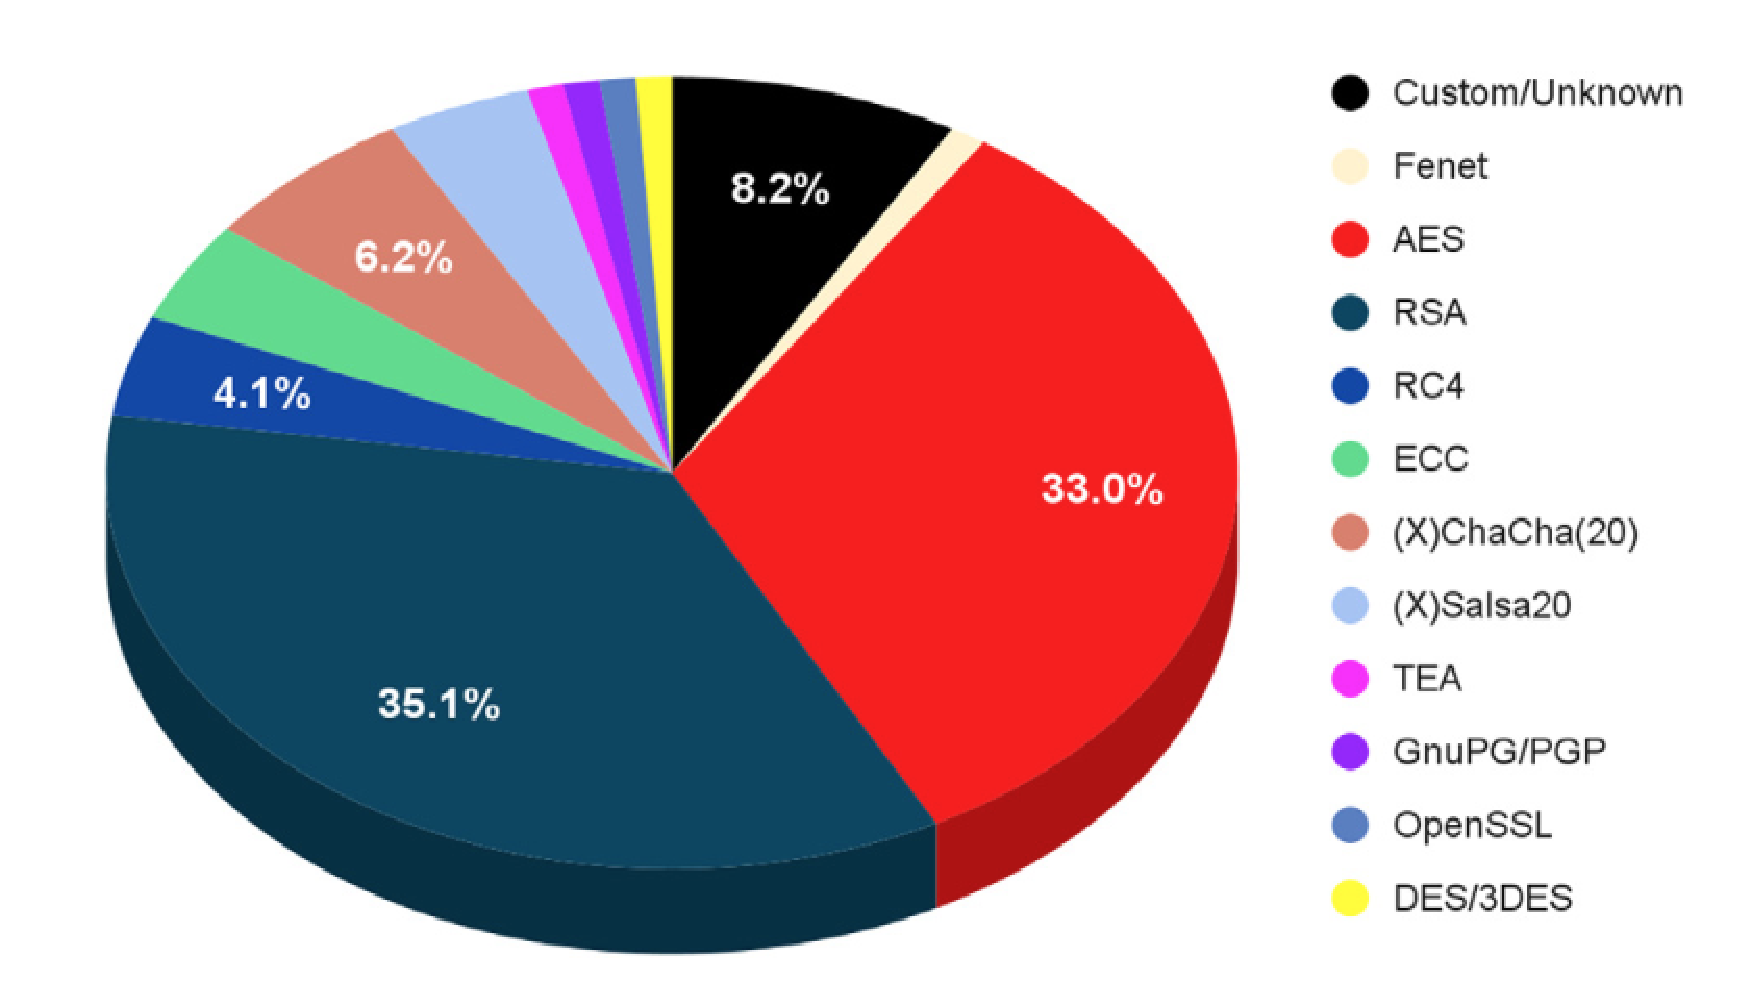
\includegraphics[width=0.8\columnwidth]{./doc/img/encrypt_algo.eps}
  \end{center}
  \caption{Breakdown of encryption algorithms used by major ransomware families (1989–2021). \cite{begovic2023cryptographic}}
  \label{fig:encrypt_algo}
\end{figure}

ランサムウェアは\textbf{対称鍵暗号化},\textbf{非対称鍵暗号化},\textbf{ハイブリッド暗号化}のいずれかの暗号化技術を採用することができる.
\\
対称鍵暗号化:
対称鍵暗号化では,暗号化と復号のために1つの鍵のみが使用される.
非対称鍵暗号化よりも高速に暗号化を行うことができるが,被害者が鍵を入手してファイルを復号することができる可能性がある.
例えば,PayBreak \cite{kolodenker2017paybreak} は,暗号化機能を提供するWindows APIの関数をフックして
暗号化に使用される共通鍵を取得することで復号を可能にしている.
そのため攻撃者は,鍵が被害者からアクセスできないようにする必要がある.
\figref{fig:encrypt_algo}より,ランサムウェアが採用する対称鍵暗号化アルゴリズムとしてはAESが
最も人気であることがわかる.
\\
非対称鍵暗号化:
非対称鍵暗号化では,暗号化鍵 (公開鍵) と復号鍵 (秘密鍵) の2つの鍵が使用される.
被害者が公開鍵を入手しても暗号化されたデータを復号することはできないため,対称鍵暗号化に比べて暗号化速度は劣るが,
暗号化鍵の保護を行う必要がない.
常に同一の鍵ペアを使用する場合,一度秘密鍵が漏洩 (または,ある被害者が身代金を支払って秘密鍵を取得)すると,その鍵ペアで暗号化されたデータは全て解読可能となる.
そのためCryptoLocker \cite{liao2016behind}などの一部のランサムウェアは,被害者ごとに異なる鍵ペアを生成する戦略を採用している.
RSAが最も頻繁に,楕円曲線暗号が次いで使用されていることが\figref{fig:encrypt_algo}よりわかる.
\\
ハイブリッド暗号化:
ハイブリッド暗号化では,
対称鍵暗号を用いてデータを暗号化した後,その暗号化鍵を非対称鍵暗号化アルゴリズムを用いて暗号化する.
これにより大量のデータの暗号化を効率よく実行しつつ,対称鍵暗号化における問題点であった鍵の保護を解決することができる.
近年の著名なランサムウェアはハイブリッド暗号化を採用しているものが非常に多い \cite{begovic2023cryptographic}.
代表例としてはWannaCry \cite{WannaCry} やCTBLocker \cite{ctb-locker} が挙げられる.

\subsection{暗号化の対象に基づく分類}
ランサムウェアはOS上でユーザが扱うデータファイル (e.g. .docx, .xlsx, .jpg) を暗号化することが一般的であるが,
ファイル以外の単位で暗号化を行うランサムウェアも存在する.
Mamba \cite{mamba-petya} はハードディスク全体を暗号化したのち
マスターブートレコード (MBR) を書き換えてOSの正常な起動を阻害し,OS起動時にランサムノートが表示されるようにする.
また,Petya \cite{mamba-petya} はWindowsシステムのマスターファイルテーブル (MFT)
\footnote{MFTはWindowsシステム内に存在するファイルの物理的な位置,ファイル名,作成者などのメタデータを管理するデータ構造である.}
を暗号化することでファイルのアクセスを不可能にする.
DarkSide \cite{DarkSide42:online} はVMWare ESXi \cite{VMwarevS52:online}
のホストマシン上で実行される.DarkSideは実行中の仮想マシン (VM) を強制終了させ,VMの仮想ディスクなどの関連ファイルを暗号化する.
これらのファイルは,典型的には\texttt{/vmfs/volumes}ディレクトリ以下のファイルであるが,
仮想マシンからは認識できない.

今日のクラウドサービスの隆盛に伴い,クラウド環境を対象としたランサムウェア攻撃が増加している.
ALIBABA Cloudの仮想ストレージサービスは2023年の第三四半期のみで1000件以上の被害報告をユーザから受けており,
2021年と比較して118\%の増加率を示している \cite{wang2024ransom}.
さらにZscaler社  は,クラウドサービスやクラウド上のワークフローに最適化されたランサムウェア
が開発されることを予測\cite{zscaler-ransomware}しており,
新しいタイプのランサムウェアの出現に備える必要がある.

